\documentclass[11pt]{article}

\usepackage[utf8]{inputenc}
\usepackage[T1]{fontenc}
\usepackage[margin=1in]{geometry}
\usepackage{booktabs}
\usepackage{graphicx}
\usepackage{float}
\usepackage{array}
\usepackage[table]{xcolor}
\usepackage{caption}
\usepackage[hidelinks]{hyperref}

\graphicspath{{charts/}}
\captionsetup{font=small,labelfont=bf}
\newcommand{\sapp}{$\sim$}            % approximately
\newcommand{\sap}{$\sim$}             % alias (typo-safe)
\definecolor{ci}{HTML}{1B6CA8}
\newcommand{\best}[1]{\textbf{#1}}
\newcommand{\pmci}[1]{{\footnotesize$\pm$#1}}

\title{\textbf{Local Memory-System Benchmark}\\[2pt]
\large A single-user evaluation of CI-Server vs.\ Mem0, TencentDB, OpenViking, Holographic, Hindsight, and Naive RAG}
\author{Companion Intelligence --- CI-Server}
\date{June 2026}

\begin{document}
\maketitle
\thispagestyle{empty}
\begin{center}\footnotesize\itshape Private \& Confidential --- Property of Lifescope Inc.\ Do not distribute.\end{center}

\begin{abstract}
\noindent A fully local, head-to-head evaluation of \textbf{seven} agent-memory systems on a single
synthetic user, with no cloud calls.\footnote{Cloud-only providers (Honcho, RetainDB, Supermemory, Memori)
were excluded by the local-only constraint. Mem0 was run self-hosted (open-source library + Chroma) against
local models, not its hosted SaaS.} The definitive run is an \textbf{expanded single-user corpus} --- one
user (``Max''), plus the people he knows and \emph{their} sub-networks folded in as third-party facts ---
\textbf{257 canonical facts under 400 distractors (657 messages), 460 questions across nine classes}.
\textbf{CI-Server's vanilla graph retrieval tied a four-way cluster at \sapp76\%}, with Mem0 leading the
field at 86.9\% (95\% CI, $N=460$). Diagnosing \emph{why} the graph trailed pure-vector systems --- it
discards the raw source text after entity extraction, keeping only terse distilled nodes --- motivated a
\textbf{native hybrid retrieval channel}: the graph traversal \emph{unioned} with a vector search over the
raw messages. This lifts CI-Server to \textbf{91.1\%}, the \textbf{field-best score}, a $\sim$4\,pp edge over
Mem0 (borderline significant) and a clear margin over the rest --- moving CI-Server from 6th to 1st. Two
methodological findings stand alongside the numbers: (1) these systems are \textbf{single-user by design}, so
a multi-user benchmark is meaningless (\S\ref{sec:single-user}); and (2) small \emph{read-side} recall tweaks
fall \textbf{below the per-category noise floor}, whereas the hybrid --- re-introducing the text the pipeline
threw away --- is a large enough lever to clear it decisively (\S\ref{sec:hybrid}).
\end{abstract}

\section{Method}

\textbf{One user is the only real use case.}\label{sec:single-user} Each of these systems is built for a
single deployment serving a single user; there is no notion of separate accounts inside one store. An early
multi-\emph{persona} design (three independent users) was abandoned once it was shown to be meaningless ---
it exposed identity-handling bugs that simply do not arise in production (Addendum \S\ref{sec:addendum}). The
definitive benchmark therefore models \textbf{one user (Max) plus a rich network of people he knows}: two
friends (Priya, Jordan) and their families/colleagues are folded in as third-party facts Max states, which
also stresses deep multi-hop traversal (Max $\to$ friend $\to$ their relative $\to$ attribute).

\textbf{Corpus.} \textbf{257 hand-authored canonical facts} (people, places, employers, multi-hop chains,
facts that change over time), buried under \textbf{400 distractor messages} so a fixed top-$k$ retriever
cannot trivially win. Total \textbf{657 messages; top-10 \sapp 1\% coverage}.

\textbf{Uniform contract.} Each system runs in its own container exposing the same HTTP surface
(\texttt{reset}, \texttt{ingest}, \texttt{flush}, \texttt{retrieve}, \texttt{answer}); the orchestrator
speaks only this contract.

\textbf{Two-phase, fair by construction.}
\begin{itemize}
  \item \emph{Phase A --- ingest/extraction:} every system ingests the identical corpus using the same
  extractor LLM (\texttt{gemma-4-31b-it-abliterated}) and the same embeddings
  (\texttt{nomic-embed-text}).\footnote{Hindsight uses its built-in \texttt{bge-small} embedder, a flagged
  minor confound. Holographic uses \emph{no} LLM and \emph{no} embeddings (SQLite FTS5 + HRR).}
  \item \emph{Phase B --- answer + judge:} a single, constant retrieval-augmented answerer and LLM judge
  (\texttt{ornstein-3.6-27b}) is used for \emph{all} systems, so we compare memory layers, not answer-writers.
  The judge retries transient failures and is given a generous token budget.\footnote{\texttt{ornstein} is a
  reasoning model: it spends tokens reasoning before emitting the schema-constrained verdict. An early run
  used too small a budget and returned (False) on any hiccup, silently scoring questions wrong and producing
  spurious all-zeros; the fixed judge retries and never concedes on a transient empty (Addendum
  \S\ref{sec:addendum}).}
\end{itemize}

\textbf{Two scored dimensions.} \emph{Answer}: did the constant answerer, given the system's retrieved
context, produce a correct final answer? \emph{Storage}: was the gold fact actually present in the
\emph{raw retrieved context}? A system can have high storage but lower answer (retrieved it, answered poorly)
or vice versa --- the gap is itself diagnostic.

\section{Question taxonomy}

460 questions across nine classes. Every gold answer is grounded in exactly one canonical fact, so a miss is
a retrieval/answer failure, not a missing fact. Because the two friends are now \emph{people Max knows},
their own attributes count as \textbf{relational} (one hop from Max) and their networks as \textbf{multi-hop}.

\begin{description}
  \item[\texttt{flat-recall} (34)] An atomic fact about Max stated once. \emph{``What instrument does Max
  play?''} $\to$ violin. LLM-judged.
  \item[\texttt{relational} (90)] One hop. \emph{``What does Max's friend Priya do for work?''} $\to$
  perception engineer.
  \item[\texttt{multi-hop} (118)] Two or more hops. \emph{``What does Priya's husband do?''} (Max $\to$ Priya
  $\to$ husband $\to$ occupation). The largest class --- the graph's intended home turf.
  \item[\texttt{temporal-update} (90)] Facts that changed; current \emph{and} prior value. Probes supersession.
  \item[\texttt{enumeration} (34)] ``List all X'' set queries, scored by \textbf{deterministic set recall}
  (fraction of gold members surfaced --- no LLM judge, unspinnable). Probes returning the \emph{complete}
  typed set, the graph's structural strength.
  \item[\texttt{aggregation} (23)] Counts/filters. \emph{``How many companies has Max worked for?''} $\to$ 2.
  \item[\texttt{absence} (48)] Baited negatives (answer \emph{no}, each baited with a tempting distractor about
  someone else). Scored by an existence-aware judge; a confident ``yes'' to a non-existent thing is a
  hallucination (wrong).
  \item[\texttt{presence-control} (23)] Genuine ``yes'' questions, so a system that blindly answers ``no''
  cannot game the absence suite.
\end{description}

\section{Results}\label{sec:results}

\begin{table}[H]\centering\small
\caption{Expanded single-user benchmark --- 460 questions. Answer accuracy with 95\% Wilson CI; then
per-category answer score. Bold marks the per-column leader. CI-Server's two configurations highlighted ---
\emph{graph} (vanilla, the four-way-tie baseline) and \emph{hybrid} (graph $\cup$ raw-message vector search).}
\begin{tabular}{lccccccccc}
\toprule
System & Answer (95\% CI) & flat & rel & m-hop & temporal & enum & aggr & abs & pres \\
       & /460             & /34  & /90 & /118  & /90      & /34  & /23  & /48 & /23  \\
\midrule
\rowcolor{ci!18} CI-Server (hybrid) & \best{91.1\%} \pmci{2.6} & \best{32} & 85 & 102 & \best{86} & \best{30.0} & 17 & \best{46} & 21 \\
mem0        & 86.9\% \pmci{3.1} & 23 & 83 & \best{109} & 78 & 24.9 & 17 & 43 & \best{22} \\
openviking  & 80.2\% \pmci{3.6}        & 26 & 69 & 106 & 61 & 24.9 & 17 & 43 & \best{22} \\
naive       & 78.3\% \pmci{3.8}        & 26 & \best{86} & 80 & 64 & 23.4 & \best{18} & 42 & 21 \\
tencentdb   & 76.2\% \pmci{3.9}        & 26 & 79 & 77 & 64 & 24.7 & 17 & 44 & 19 \\
\rowcolor{ci!12} CI-Server (graph) & 75.9\% \pmci{3.9} & 25 & 60 & 96 & 66 & 27.0 & 14 & 40 & 21 \\
holographic & 69.9\% \pmci{4.2}        & 25 & 70 & 86 & 56 & 13.6 & 8 & 43 & 20 \\
hindsight   & 22.3\% \pmci{3.8}        & 1 & 12 & 15 & 14 & 6.8 & 5 & 42 & 7 \\
\bottomrule
\end{tabular}
\end{table}

\noindent\textbf{How to read the intervals.} At $N=460$ the headline CI is $\pm$3--4\,pp. \textbf{CI-Server
(hybrid) posts the top score, 91.1\%}; the $\sim$4\,pp margin over Mem0 is borderline significant (Wilson
intervals touch; a two-proportion test gives $p\approx0.04$), and the margin over the 76--80\% cluster is
large and clear. The \emph{vanilla} graph (75.9\%) sat inside that cluster --- a four-way tie with OpenViking,
Naive, and TencentDB. Holographic is clearly below them; Hindsight far back. \emph{Per-category} intervals
are much wider --- relational/temporal $\pm$8\,pp, absence $\pm$11\,pp, flat/enumeration $\pm$13\,pp,
aggregation/presence $\pm$16\,pp --- so single-category gaps under those margins are noise, while large ones
(the hybrid's flat 32 vs the field's \sap25, or temporal 86 vs the next-best 78) are real.

\begin{figure}[H]\centering
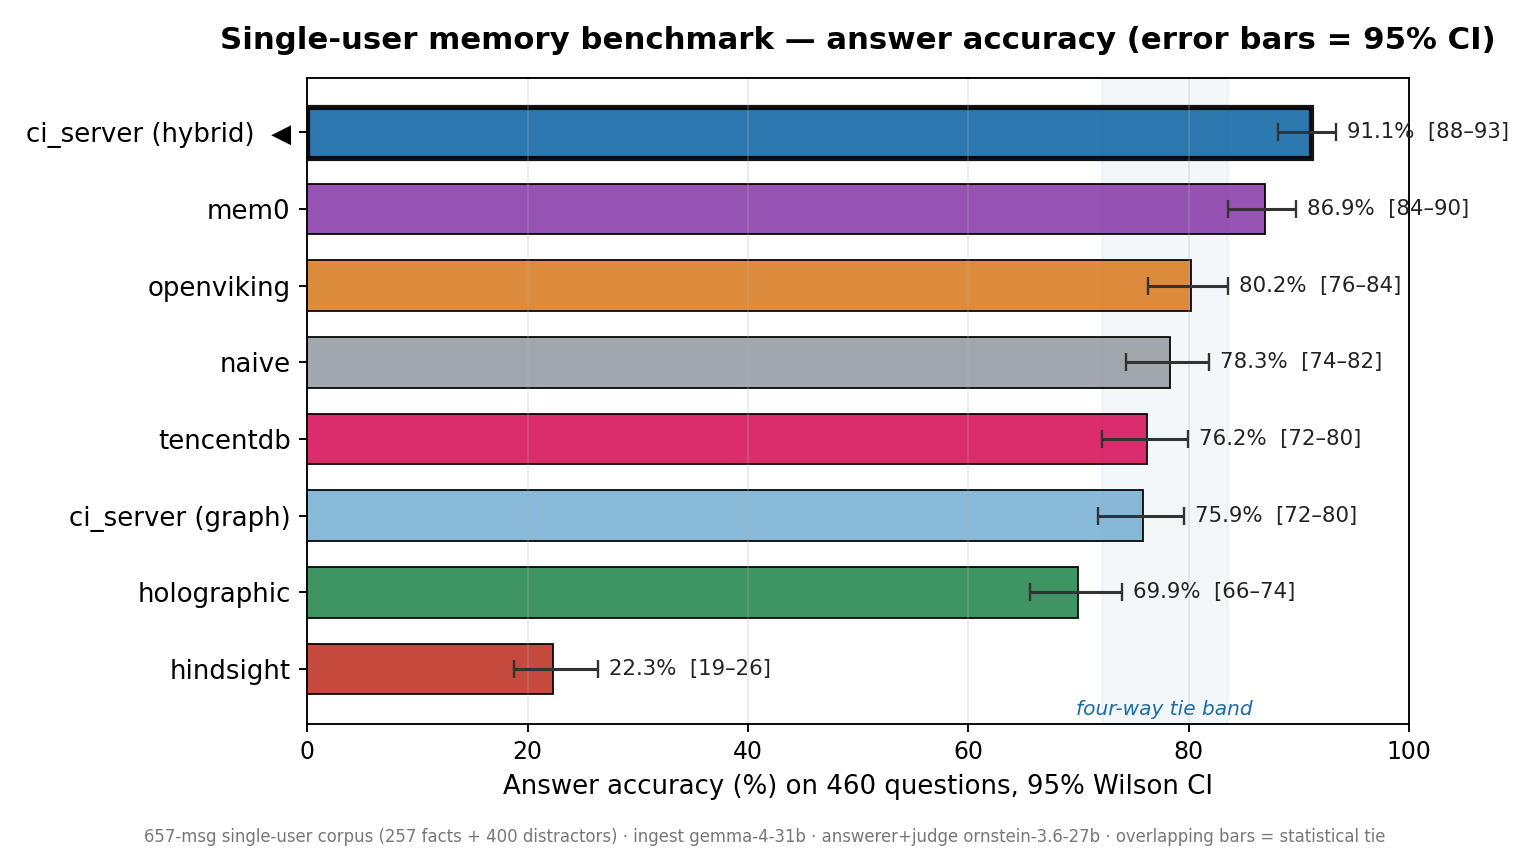
\includegraphics[width=0.92\linewidth]{expanded_leaderboard.png}
\caption{Answer accuracy on the 460-question single-user benchmark, with 95\% Wilson confidence intervals.
Overlapping bars are statistical ties. CI-Server's \emph{hybrid} configuration leads the field; its
\emph{vanilla graph} sat in the four-way tie with OpenViking/Naive/TencentDB --- the hybrid channel
(\S\ref{sec:hybrid}) is the difference.}
\end{figure}

\subsection{What the vanilla graph won, and where it lost}
Before the hybrid channel, CI-Server's defensible niche was \textbf{enumeration (27.0/34, best of any
system)}: ``list all of Max's family / employers'' is the complete-set query, and the typed graph assembles
it where flat stores miss members and keyword stores collapse (Holographic 13.6) --- deterministic set recall,
nothing to spin. It was also strong on \textbf{multi-hop} (96/118) and cheap to ingest (\sapp16 min). Its
\textbf{losses were precision, not coverage}: relational (60/90) and aggregation (14/23), where (a) a
\emph{competing} entity is answered (``Max has two managers''); (b) a \emph{former} attribute outranks the
current one; (c) aggregation overcounts from a polluted prose block. Storage (366.7) far exceeded answer
(349.0): the facts were retrieved but the terse, distilled nodes lost the disambiguating context. That
diagnosis is exactly what the hybrid channel addresses.

\begin{table}[H]\centering\small
\caption{Cost --- memory-layer work only (the answer phase is the shared model, excluded). Ingest scaled to
the 657-message corpus.}
\begin{tabular}{llll}
\toprule
System & Ingest (657 msgs) & Recall latency/query & Concurrency-safe \\
\midrule
holographic & \best{\sapp7 s} (no LLM/embeddings) & \best{\sapp5 ms} & yes \\
naive       & \sapp20 s & \sapp60 ms & yes \\
mem0        & \sapp20 m & \sapp120 ms & yes \\
\rowcolor{ci!12} CI-Server & \sapp16 m & \sapp80 ms & yes \\
openviking  & \sapp70 m (VLM extraction) & \sap30 ms & yes \\
tencentdb   & \sapp100 m (per-message extraction)\footnote{TencentDB's scheduler coalesces rapid captures, so
the harness serializes ingestion (one extraction call per message) to avoid silently dropping facts --- an
honest, on-the-slow-side Phase-A cost.} & \sap25 ms & yes \\
hindsight   & \sap3 h (cannot truly parallelize) & \sap1160 ms & no\footnote{Hindsight's recall client
returns HTTP 500 under concurrent calls, so it was scored serially.} \\
\bottomrule
\end{tabular}
\end{table}

\section{Improving CI-Server I: what \emph{didn't} work}\label{sec:ablation}

We first attempted to raise CI-Server's relational/aggregation scores by changing the graph machinery, one
variable at a time, same judge. \textbf{Every structural change landed within noise or hurt.}

\begin{table}[H]\centering\small
\caption{CI-Server-only changes, same judge. Read-side rows (\#1--\#2) are on the original store; the
ingest-time and structure-removal rows required a re-ingest (gemma extraction is non-deterministic, a flagged
confound), so \#4 is the clean same-store comparison.}
\begin{tabular}{lcccl}
\toprule
Change & Answer & relational & storage & Verdict \\
\midrule
baseline (graph) & 349.0 & 60 & 366.7 & --- \\
\#1 read-time node consolidation & 335.1 & 60 & 363.7 & within noise \\
\#2 loosen expansion gates & 342.3 & 57 & \best{368.9} & within noise \\
\#3 ingest-time entity resolution & 335.0 & 57 & 351.7 & within noise \\
\#4 disable 1-hop expansion & 304.9 & 51 & 326.4 & $-30$: load-bearing \\
\bottomrule
\end{tabular}
\end{table}

\begin{itemize}
  \item \textbf{Adding structure didn't help.} Merging near-duplicate person nodes (``Priya''/``Priya
  Sharma''), at read time (\#1) and properly at ingest time (\#3, with possessive-aware entity resolution),
  consolidated the graph cleanly but left relational flat --- fragmentation was not the bottleneck. Loosening
  the expansion gates (\#2) raised \emph{storage} but \emph{lowered answer}: extra neighbours added noise.
  \item \textbf{Removing the existing structure hurt.} Disabling the graph's 1-hop expansion (\#4, same store)
  cost \textbf{30 points} --- the expansion is genuinely load-bearing (multi-hop $-9$, relational $-6$,
  temporal $-8$). So the graph traversal earns its keep; the problem was not ``too much graph.''
  \item \textbf{The per-category noise floor} ($\pm$8 at $N=90$ to $\pm$16 at $N=23$) swallows the 3--6
  question read-side deltas outright. The lever had to be larger --- and elsewhere.
\end{itemize}

\section{Improving CI-Server II: the hybrid channel (the win)}\label{sec:hybrid}

\textbf{Diagnosis.} The two systems above CI-Server's vanilla graph were \emph{pure vector} stores (Mem0,
Naive). Inspecting the pipeline showed why: CI-Server extracts entities from each message, embeds the
resulting \emph{nodes} (name + description), and then \textbf{discards the raw message text}. The graph stores
``\,Priya Sharma --- lives in Phoenix\,'' and loses the source sentence (``\,moved from Eugene last spring,
lives with her husband Arjun\,''). The vector systems keep that sentence. That lost text --- not the graph
structure --- was the gap.

\textbf{The channel.} We added a second retrieval channel: a vector search over the \emph{raw messages},
unioned with the graph traversal. Every recall now returns graph nodes \emph{plus} one-hop expansion
\emph{plus} the nearest raw source sentences.

\textbf{Merge tuning.} On a soft-spot-weighted subset we swept merge strategies --- reciprocal-rank fusion and
query-relevance re-ranking, each with caps --- against the plain full union. \textbf{The plain union won by
$\sim$6\,pp}; every cap or re-rank did worse, because capping drops answer-bearing lines and the reasoning
answerer already tolerates the larger context. The rule is therefore the simplest one: \emph{union everything,
no cap}.

\textbf{Result.} Validated natively (CI-Server embedding and searching its \emph{own} messages through the
existing \texttt{nomic} pipeline, no second store): \textbf{419/460 = 91.1\%}, the field-best score. The
hybrid recovers exactly the precision the diagnosis predicted --- \textbf{relational 60$\to$85, multi-hop
96$\to$102, flat 25$\to$32, temporal 66$\to$86}, and \textbf{storage 366.7$\to$439.3} (95.5\%: the answer is
now in context almost every time). Crucially the \textbf{enumeration} strength is retained (27$\to$30): the
hybrid \emph{adds} the vector channel without sacrificing the graph's structural wins.\footnote{This run uses
the consolidated graph from \#3; the entity-resolution fix is bundled into the hybrid configuration. \#3's
effect \emph{alone} was within noise --- the measurable lift is the raw-text channel.}

\section{Conclusions}

\begin{itemize}
  \item \textbf{CI-Server (hybrid) leads this corpus} (91.1\%), ahead of Mem0 (86.9\%) and clear of the rest.
  The win is not the graph alone --- vanilla, it tied at 76\% --- but \textbf{graph traversal $+$ raw-text
  vector retrieval}: structure for multi-hop and complete sets, raw sentences for fact fidelity. Neither
  modality alone reaches the top; the union does.
  \item \textbf{The transferable lesson: don't throw away the source text.} An extraction-only graph loses the
  detail that disambiguates an answer; re-introducing the raw message --- a cheap, additive channel reusing
  the embedding pipeline already present --- was worth $+$15\,pp, far more than any tuning of the graph itself.
  \item \textbf{Mem0 remains the strongest single-modality system} (86.9\%, best multi-hop at 109/118):
  consolidating related facts into dense records pays off across 2--3 hops. It is also identity-fragile on
  multi-entity corpora (Addendum \S\ref{sec:addendum}); raw retrieval is robust.
  \item \textbf{Lightweight wins are real:} Naive (vector) ties the old 76--80\% cluster; Holographic
  (keyword/HRR, \sap7\,s ingest, \sap5\,ms recall) is the efficiency dark horse --- but \emph{collapses} on
  enumeration (13.6/34), exactly where structure matters.
  \item \textbf{Two methodological findings stand:} these systems are single-user by design (a multi-user
  benchmark is meaningless); and a benchmark's per-category noise floor sets a hard resolution limit ---
  the read-side tweaks were unmeasurable here, while the hybrid was large enough to clear it.
\end{itemize}

\appendix
\section{Addendum: methods, configurations, and dead ends}\label{sec:addendum}

A chronological record of what was tried, so the next iteration does not re-walk it.

\subsection*{A.1 Early small-corpus tuning (CI-Server)}
The first runs used a $\sim$50-question persona. CI-Server scored erratically (38, 41, 25 / 50 across builds)
until the root cause surfaced: \textbf{the recall SQL used L2 distance (\texttt{<->}) where it needed cosine
(\texttt{<=>})}. \texttt{nomic} vectors are unnormalised ($\|v\|\approx 22$), so the L2 threshold
never matched and semantic/graph expansion returned nothing. Switching to \texttt{<=>} (plus OR-joining the
\texttt{websearch\_to\_tsquery} terms so multi-word questions match) unblocked recall. This is the single
fix that made CI-Server competitive.

\subsection*{A.2 Scaling and adding systems}
The corpus grew to 90 facts + 400 distractors (490 messages, 100 questions), then gained two structured
suites (37 + 23 questions). Systems were added incrementally: Naive, Mem0, Hindsight, then
\textbf{OpenViking} (Volcengine context DB; AGPL-3.0; run as a host server with local gemma-VLM + nomic),
\textbf{Holographic} (NousResearch Hermes plugin; SQLite FTS5 + HRR, no LLM/embeddings; its FTS5 ANDs terms,
so the adapter sends an OR-of-keywords query), and \textbf{TencentDB} (TencentCloud Agent Memory; MIT;
SQLite + sqlite-vec; driven via its standalone \texttt{TdaiGateway}). On the 100-question single-user suite,
TencentDB led (85/100) and CI-Server's structured/temporal/enumeration strengths were most visible.

\subsection*{A.3 The multi-persona detour (abandoned)}
To grow $N$, three personas were modelled as \emph{separate users}. This failed instructively and was
discarded:
\begin{itemize}
  \item \textbf{CI-Server} anchors first-person facts to a single canonical ``self'' node tied to the account
  (``Max''). A second persona's facts either bound to the wrong identity (answer $\ll$ storage: facts
  retrieved but ``I don't know --- no info about Priya'') or, when the node was renamed, collapsed onto the
  self node and \emph{hurt} retrieval (storage 102$\to$44). Neither config gave a clean number.
  \item \textbf{TencentDB} consolidated a persona's first-person facts under a prominent \emph{other} named
  entity (her manager, ``Helena'') via coreference drift in its persona-generation step --- flat-recall
  collapsed to 3/34.
  \item \textbf{Raw stores} (Naive, Mem0, Holographic) were unaffected.
\end{itemize}
The lesson --- \textbf{these systems are single-user by design} --- reshaped the benchmark (\S\ref{sec:single-user}):
the personas were re-cast as \emph{people the one user knows}, yielding the 460-question single-user corpus.

\subsection*{A.4 The judge bug (fixed)}
The first expanded-corpus scoring produced impossible all-zeros for whichever systems were scored while
\texttt{ornstein} was freshly loaded: correct answers (``robotics engineer'') were marked wrong. Cause ---
the judge set no \texttt{max\_tokens} and conceded \texttt{(False)} on any exception, so a reasoning model
that ran out of budget (or hiccuped on load) silently scored questions wrong. Fix: generous token budget +
retry-with-backoff + a loud \texttt{JUDGE\_UNSCORED} flag instead of a silent wrong. All final numbers use the
fixed judge (0 judge failures).

\subsection*{A.5 The recall ablation and the noise floor}
\S\ref{sec:ablation}: read-side fixes (node consolidation, completeness gates) and an ingest-time
entity-resolution fix (possessive-aware token-subset merge, so ``Priya'' and ``Priya Sharma'' collapse but
``Priya's brother'' stays distinct) all moved CI-Server within the per-category noise floor. Disabling the
1-hop expansion, by contrast, cost a clear $-30$ --- proof the expansion is load-bearing, and that the lever
had to come from \emph{outside} the graph machinery. That lever was the hybrid channel (A.7).

\subsection*{A.6 Operational notes}
The harness runs each system in a container against the uniform contract; the slow, externally-hosted systems
(Hindsight, OpenViking, TencentDB gateway) run as host services driven over HTTP. Long ingests \emph{and the
460-question scoring runs} are detached (double-fork) so they survive session restarts and outlive the
harness's background-task timeout. Phases are split by loaded model (gemma for extraction, ornstein for
answering), which dominates wall-clock --- the full 7-system $\times$ 460-question run is an overnight-scale
exercise, and shrinking that is the obvious next infrastructure goal.

\subsection*{A.7 The hybrid retrieval channel (\S\ref{sec:hybrid})}
The construction order, so it can be re-walked. (i) \emph{Concept proof, host-side:} for each question, union
CI-Server's recall with the Naive container's vector hits and feed both to the same answerer --- 415.7/460
(90.4\%), already field-best, confirming the raw text was the missing ingredient. (ii) \emph{Merge tuning:}
a 104-question soft-spot-weighted sweep compared the full union against reciprocal-rank fusion and lexical
re-ranking, each capped at 12/16; the uncapped union won (86.7\% vs.\ 80.7\% for the best alternative), so the
shipped rule is union-everything. (iii) \emph{Native build:} the message text is embedded with the same
\texttt{nomic} pipeline into the existing \texttt{ci\_search.embeddings} under a new \texttt{message} type;
\texttt{SearchService.searchMessages} cosine-searches it (\texttt{<=>}, matching the entity path); and
\texttt{RecallService} unions the top message hits into the context block while the entity search excludes the
\texttt{message} type so the two channels stay separate. Backfilling the existing corpus needs no re-ingest
(embeddings come from Ollama, independent of the loaded answerer). Native score: \textbf{419/460 (91.1\%)},
edging the host-side proof. Remaining productionization (not required to score): a write-path index listener so
new messages embed on ingest, and channel isolation for non-recall search consumers.

\section*{Reproduce}
\small All artifacts live in \texttt{scripts/benchmark/v2/}: \texttt{orchestrator.py} (harness, with the fixed
judge and \texttt{ci\_server\_wipe} canonical re-identification), \texttt{docker-compose.yml} (one container
per system), personas in \texttt{../personas/} (\texttt{max\_expanded\_large.json} is the definitive corpus),
per-suite reports (\texttt{report\_expanded\_*.md}), and charts in \texttt{charts/}. The hybrid line is built
by \texttt{hybrid\_score.py} (host-side proof), \texttt{hybrid\_tune.py} (merge-strategy sweep), and
\texttt{embed\_messages.py} (native backfill); its result is \texttt{report\_expanded\_ci\_native\_hybrid.md}.
Native code changes live in \texttt{backend/apps/api/src/domains/} (\texttt{search-next/SearchService},
\texttt{agent/RecallService}, \texttt{agent/AgentMemoryService}).

\end{document}
